\chapter{Electricity Fundamentals}
\label{ch:electricity}

\section{Charge, Current, and the Electron}

All electrical phenomena trace back to \textbf{electric charge}, a
fundamental property of matter carried by protons (positive) and
electrons (negative). Charge is measured in \textbf{coulombs (C)}. In
solid conductors, current flow is due almost entirely to the drift of
free electrons through the material's crystal lattice; each electron
carries a charge of
\[
e = 1.602 \times 10^{-19}\,\text{C}.
\]

\textbf{Electric current}, symbol $I$, is defined as the rate of flow of
charge past a point:
\[
I = \frac{Q}{t} \qquad [\text{amperes, A}]
\]
where $Q$ is the charge in coulombs that passes in time $t$ (seconds). One
ampere is one coulomb per second. Rearranged, this gives $Q = It$, used
whenever you need to know how much charge (and hence how much battery
capacity) a circuit consumes over time.

\begin{keyidea}[Conventional current vs.\ electron flow]
By historical convention (fixed before the electron was discovered),
current is defined as flowing from the positive terminal of a source,
through the external circuit, to the negative terminal. Electrons
actually drift the opposite way. Every formula and every schematic
arrow in this book uses \emph{conventional current}; keep this in mind
if you ever reason from first-principles electron motion.
\end{keyidea}

\section{Voltage: Electromotive Force and Potential Difference}

\textbf{Voltage} (potential difference), symbol $U$ or $V$, is the energy
per unit charge available to move charge between two points:
\[
U = \frac{W}{Q} \qquad [\text{volts, V}]
\]
where $W$ is energy in joules and $Q$ is charge in coulombs. A source that
maintains a potential difference by chemical, mechanical, or
photovoltaic means (a battery, generator, or solar cell) is said to
supply an \textbf{electromotive force (EMF)}. Voltage is always measured
\emph{between two points} --- it is meaningless to speak of ``the voltage
at a point'' without an implied reference (commonly circuit ground, 0\,V).

\section{Resistance and Conductance}

\textbf{Resistance}, symbol $R$, measured in \textbf{ohms ($\Omega$)},
quantifies how strongly a material opposes current flow. Its reciprocal,
\textbf{conductance} $G = 1/R$, is measured in \textbf{siemens (S)} and is
occasionally more convenient when components are combined in parallel
(Chapter~\ref{ch:dc-circuits}).

The resistance of a uniform conductor depends on its physical dimensions
and the material's intrinsic \textbf{resistivity} $\rho$ (ohm-metres):
\[
R = \rho\,\frac{\ell}{A}
\]
where $\ell$ is the conductor's length and $A$ its cross-sectional area.
This equation explains several practical facts amateurs rely on: thicker
wire has lower resistance (larger $A$), longer feedlines have more loss
(larger $\ell$), and different metals used for antenna elements or wire
(copper, aluminum, steel) behave differently because of $\rho$.

Resistance also depends on temperature. For most conductors, resistance
\emph{increases} with temperature (a fact relevant to power resistors and
antenna tuner components that heat up under load); for semiconductors, it
typically \emph{decreases}, a behavior exploited in some temperature
sensors.

\section{Ohm's Law}
\label{sec:ohms-law}

The single most-used relationship in all of electronics is \textbf{Ohm's
law}, named for Georg Simon Ohm (1789--1854):
\[
\boxed{U = IR}
\]
Voltage equals current multiplied by resistance. Because it relates three
quantities, knowing any two lets you solve for the third:
\[
I = \frac{U}{R}, \qquad R = \frac{U}{I}.
\]

\begin{center}
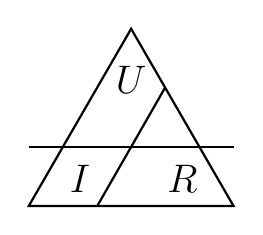
\begin{tikzpicture}[scale=1]
\draw[thick] (0,0) -- (2.6,0) -- (1.3,2.25) -- cycle;
\draw[thick] (0,0.75) -- (2.6,0.75);
\draw[thick] (0.87,0) -- (1.73,1.5);
\node at (1.3,1.6) {\Large $U$};
\node at (0.65,0.35) {\Large $I$};
\node at (1.95,0.35) {\Large $R$};
\end{tikzpicture}
\end{center}

The classic memory triangle above encodes all three rearrangements: cover
the quantity you want to find, and the remaining two show whether to
multiply or divide. Covering $U$ leaves $I$ beside $R$ (multiply, $U=IR$);
covering $I$ leaves $U$ over $R$ (divide, $I=U/R$); covering $R$ leaves
$U$ over $I$ (divide, $R=U/I$).

\begin{center}
\begin{tabular}{@{}llll@{}}
\toprule
Quantity & Symbol & Unit & Symbol for Unit \\
\midrule
Voltage (potential difference) & $U$ & volt & V \\
Current & $I$ & ampere & A \\
Resistance & $R$ & ohm & $\Omega$ \\
\bottomrule
\end{tabular}
\end{center}

\begin{examplebox}[Applying Ohm's law]
A 12\,V battery is connected across a 470\,$\Omega$ resistor. Find the
current.

\emph{Solution.}
\[
I = \frac{U}{R} = \frac{12\,\text{V}}{470\,\Omega} = 0.0255\,\text{A} = 25.5\,\text{mA}.
\]
\end{examplebox}

\begin{examtip}
Ohm's law questions on exams almost always require a prefix conversion as
part of the arithmetic (mA, k$\Omega$, etc.). Convert everything to base
units (V, A, $\Omega$) first, solve, then convert the final answer to a
sensible prefix.
\end{examtip}

\section{Electrical Power}

\textbf{Power} is the rate of doing work (transferring energy), measured
in \textbf{watts (W)}:
\[
P = \frac{W}{t}.
\]
In a DC circuit, electrical power delivered to a component is
\[
\boxed{P = UI}
\]
Combining this with Ohm's law gives two further useful forms, used
whenever voltage or current (rather than both) is known:
\[
P = I^{2}R, \qquad P = \frac{U^{2}}{R}.
\]

\begin{examplebox}[Power dissipation]
The 470\,$\Omega$ resistor from the previous example carries 25.5\,mA.
How much power does it dissipate, and could a standard $\tfrac{1}{4}$-W
resistor be used safely?

\emph{Solution.}
\[
P = I^2 R = (0.0255\,\text{A})^2 \times 470\,\Omega \approx 0.306\,\text{W}.
\]
This exceeds a $\tfrac{1}{4}$-W (0.25\,W) resistor's rating, so a
$\tfrac{1}{2}$-W or larger resistor should be used, ideally with margin
for safety (Section~\ref{sec:power-derating}).
\end{examplebox}

\begin{safetynote}[Power rating margin]
Never operate a resistor, or any dissipative component, right at its
rated maximum. A common engineering rule of thumb is to keep steady-state
dissipation below 50\% of the component's rating, both because
resistance itself drifts with temperature and because localized hot spots
can exceed the average calculated value.
\label{sec:power-derating}
\end{safetynote}

\section{Energy}

Energy is power sustained over time:
\[
W = Pt.
\]
When $P$ is in watts and $t$ is in seconds, $W$ comes out in joules.
Utility bills and battery capacities, however, are usually expressed in
\textbf{watt-hours (Wh)} or \textbf{kilowatt-hours (kWh)}, where $t$ is in
hours instead of seconds; $1\,\text{kWh} = 3.6\times10^{6}\,\text{J}$.
Battery amp-hour ratings, covered in Chapter~\ref{ch:power-sources}, use
the same underlying idea applied to charge instead of energy.

\section{Conductors, Insulators, and Semiconductors}

Materials are broadly classed by how easily their electrons can move
under an applied field:

\begin{itemize}
\item \textbf{Conductors} (copper, aluminum, silver, gold) have a ``sea''
of loosely bound valence electrons that move freely, giving very low
resistivity ($\rho \sim 10^{-8}\,\Omega\cdot\text{m}$). Used for wire,
antenna elements, PCB traces.
\item \textbf{Insulators} (PVC, ceramic, glass, air under normal
conditions) have tightly bound electrons and extremely high resistivity
($\rho \sim 10^{9}$--$10^{16}\,\Omega\cdot\text{m}$). Used to prevent
unwanted current paths --- wire jacketing, standoff insulators, capacitor
dielectrics.
\item \textbf{Semiconductors} (silicon, germanium) have resistivity
between the two, and --- crucially --- that resistivity can be controlled
by doping, temperature, or an applied field. This tunability is what
makes diodes, transistors, and integrated circuits possible
(Chapter~\ref{ch:semiconductors}).
\end{itemize}

\begin{quickreview}
\item Current $I = Q/t$; voltage $U = W/Q$; resistance $R = U/I$ (Ohm's
law, $U = IR$).
\item Conventional current flows from $+$ to $-$ through the external
circuit, opposite to actual electron drift.
\item $R = \rho \ell / A$: resistance rises with length, falls with
cross-sectional area, and depends on material resistivity.
\item Power: $P = UI = I^2R = U^2/R$; energy $W = Pt$.
\item Conductors, insulators, and semiconductors are distinguished by
resistivity and by whether that resistivity can be externally controlled.
\end{quickreview}

\begin{practiceproblems}
\item A 9\,V battery drives 300\,mA through a resistor. Find the
resistance.
\item Find the power dissipated by a 100\,$\Omega$ resistor carrying
50\,mA.
\item A device draws 2\,A at 13.8\,V for 3 hours. How much energy, in
watt-hours, did it consume?
\item A wire's length is doubled and its cross-sectional area is halved.
By what factor does its resistance change?
\item Explain, using the concept of resistivity, why thick antenna
feedline conductors have less loss than thin ones of the same length.
\end{practiceproblems}
